%!TEX root = paper.tex
\section{Background}
\label{sec:background}
This section presents some preliminary knowledge about
statistical inference and, in particular, Bayesian inference using 
variational message passing, a popular variational inference algorithm, 
as well as its implementation concerns on Apache Spark/GraphX stack.
  
\subsection{Statistical Inference}

Statistical inference is a common machine learning task of obtaining the
properties of the underlying distribution of data. For example, one can infer
from many coin tosses the probability of the coin turning up head by counting
how many tosses out of the all tosses are head. There are two different
approaches to model the number of heads: the frequentist approach and the
Bayesian approach.


Let $N$ be the total number of tosses and $H$ be the number of heads.  In
frequentist approach, the probability of coin turning up head is viewed as an
unknown \emph{fixed} parameter so the best guess $\phi$ would be the number of heads $H$ in the
results over the total number of tosses $N$.
\begin{equation*}
	\phi = \frac{H}{N}
\end{equation*}

In Bayesian approach, the probability of head is viewed as a hidden \emph{random
variable} drawn from a prior distribution, e.g., $\mathrm{Beta}(1, 1)$, the
uniform distribution over [0, 1]. According to the Bayes Theorem, the
posterior distribution of the probability of coin turning up head can be
calculated as follows:

\begin{align*}
	p(\phi|x) &= \frac{ \phi^H (1-\phi)^{N-H} f(\phi; 1, 1)}{\int_0^1 \phi^H
	(1-\phi)^{N-H} f(\phi; 1, 1)\mathrm{d}\phi} \\ &= f(\phi; H+1, N-H+1) \numberthis
	\label{eqn:coin_posterior}
\end{align*}

\noindent
where $f(\cdot; \alpha, \beta)$ is the probability density function (PDF) of
$\mathrm{Beta}(\alpha, \beta)$ and $x$ is the outcome of $N$ coin tosses.

The frequentist approach needs smoothing and regularization techniques to
generalize on unseen data while the Bayesian approach does not because the
latter can capture the uncertainty by modeling the parameters as random
variables. 

\subsection{Probabilistic Graphical Model}

Probabilistic graphical model \cite{pgm} (PGM) is a graphical representation of the
conditional dependencies in statistical inference. Two types of PGM are widely
used: Bayesian networks and Markov networks. Markov networks are undirected
graphs while Bayesian networks are directed acyclic graphs. Each type of PGM
can represent certain independence constraints that the other cannot represent. 
InferSpark currently supports Bayesian networks and regards Markov networks 
as the next step.  
\begin{figure}[h]
	\centering
	\includegraphics[scale=0.38]{figs/one_coin.eps}
	\caption{Bayesian network of the coin flip model (observed/unobserved random
	variable are in dark/white)}
	\label{fig:coin_bn}
\end{figure}

In a Bayesian network, the vertices are random variables and the edges
represent the conditional dependencies between the random variables.
The joint probability of a Bayesian network can be factorized into conditional
probabilities of each vertex $\theta$ conditioned on their parents
$\mathrm{F}(\theta)$. 
\figref{fig:coin_bn} is the Bayesian network of the coin flip model.  
Here, the factors in the joint
probability are $p(\phi)$ and $p(x|\phi)$. The plate surrounding $x$ represents
repetition of the random variables. The subscript $N$ is the number of
repetitions. The outcome of coin tosses $x$ is repeated $N$ times and
each depends on the probability $\phi$. The Bayesian network of the coin flip
model encodes the joint probability $p(\phi, x) =
p(\phi)\prod_{i=1}^{N}p(x_i|\phi)$. 

Bayesian networks are generative models, which describes the process of
generating random data from hidden random variables. The typical inference
task on generative model is to calculate the posterior distribution of the
hidden variables given the observed data. In the coin flip model, the
observed data are the outcomes of coin tosses and the hidden random variable
is the probability of head. The inference task is to calculate the posterior
in Equation \ref{eqn:coin_posterior}.

\subsection{Bayesian Inference Algorithms}


\begin{figure}
	\centering
	\includegraphics[scale=0.4]{figs/two_coins.eps}
	\caption{Bayesian network of the two-coin model}
	\label{fig:two_coins}
\end{figure}

Inference of the coin flip model is simple because the posterior
(Equation \ref{eqn:coin_posterior})
 has a tractable analytical solution. 
However, most real-world models are more complex than that
and their posteriors do not have a familiar form. 
Moreover, even calculating the
probability mass function or probability density function at one point is hard
because of the difficulty of calculating the probability of the
observed data in the denominator of the posterior. The probability of the
observed data is also called evidence. It is the summation or integration over
the space of hidden variables and is hard to calculate because of exponential
growth of the number of terms. 

Consider a two-coin model in \figref{fig:two_coins}, where we first decide
which coin to toss, with probability $\pi_1$ to choose the first coin and
probability $\pi_2$ to choose the second coin ($\pi_1 = 1 - \pi_2$). 
We then toss the chosen coin, which has probability $\phi_i$ to turn up head. 
This process is repeated $N$ times. The two-coin model is
a {\em mixture model}, which represents the
mixture of multiple sub-populations. Each such sub-population, in this case
$\phi_1$ and $\phi_2$, have their own distributions, 
while the observation can only be obtained on the overall population, that is
the number of heads after $N$ tosses. 
The two-coin model has no tractable analytical solution. 
Assuming Beta priors for $\pi$, $\phi_{1}$ and $\phi_{2}$, 
the posterior distribution is:

{
\small
\begin{align*}
%	&p(\pi, \phi, x) = \\
%	&f(\pi)f(\phi_1)f(\phi_2)(\pi_1 \phi_1 + \pi_2 \phi_2)^H (\pi_1
%	(1-\phi_1) + \pi_2 (1- \phi_2))^{N-H} \\
	&p(\pi, \phi | x) = \frac{p(\pi, \phi, x)}{\int p(\pi, \phi, x) \dd \pi \dd
\phi_1 \dd \phi_2}
\end{align*}
}

\noindent
where the joint distribution $p(\pi, \phi, x)$ is:

{\small
\begin{align*}
%	&p(\pi, \phi, x) = \\
	&f(\pi)f(\phi_1)f(\phi_2)(\pi_1 \phi_1 + \pi_2 \phi_2)^H (\pi_1
	(1-\phi_1) + \pi_2 (1- \phi_2))^{N-H} \\
\end{align*}
}


The integral in the denominator of the posterior is intractable 
because it has $2^N$ terms and takes exponential time to compute.  
Since solving for the exact posterior is
intractable, approximate inference algorithms are used instead.
Although approximate inference is also NP-hard, it performs well in 
practical applications. 
Approximate inference techniques include Markov Chain Monte Carlo (MCMC) 
method, variational inference and so on.
%MCMC algorithms are more
%accurate than the variational inference but the running time is usually much
%longer. 
MCMC algorithms are inherently non-deterministic, and single random number
generator is required to ensure randomness. In a distributed setting, sharing
a single random number generator across the nodes in a cluster is a serious
performance bottleneck. Having different generators on different nodes would
risk the correctness of the MCMC algorithms.
On the other hand, variational inference methods such as
Variational Message Passing (VMP) \cite{vmp}
%of exponential-conjugate Bayesian networks because it
%can be expressed as a 
is a deterministic graph-based message passing algorithm, 
which can be easily adapted to a distributed graph computation model such as
GraphX \cite{graphX}. 
InferSpark currently supports VMP.
Support of other techniques (e.g., MCMC) is included in InferSpark's open-source agenda.

\begin{figure}[ht]
	\centering
	\includegraphics[scale=0.4]{figs/two_coins_latent.eps}
	\caption{Expanded Bayesian network of the two-coin model}
	\label{fig:two_coin_bn}
\end{figure}

To infer the posterior of the two-coin model using VMP,
the original Bayesian network has to be expanded by 
adding some more hidden random variables.
Figure \ref{fig:two_coin_bn}
shows Bayesian network with hidden random variables added,
%illustrate the algorithm, we use the two-coin model
%(\figref{fig:two_coin_bn}), a slightly more complex model than the one-coin
%model. 
where $z_i$ is the index (1 or 2) of the coin chosen for the $i^{th}$ toss.

%$z_{ij}$ is an indicator random variable 
%where if the $j$-th coin is chosen
%in the $i$-th experiment,   then $z_{ij} = 1$, else $z_{ij} = 0$ otherwise.
%\ERIC{am I correct here, ZY?}

%
%Let $k \in \{1, 2\}$ be the indices of the coins. Coin $k$'s probability of turning head is $\phi_k$. 
%We repeat the experiment for $N=2$ times. 
%In the $i^{th}$ experiment, we first choose
%one of the coin with probabilities $\pi_1$ and $\pi_2 = 1 - \pi_1$. 
%Let the index of the chosen coin be $z_i$. 
%Then we flip the coin $z_i$ once and get a
%head or a tail, denoted as $x_i$. For any of the variables $v$ above, we use
%$v_j, j \in \dom(v)$ as an indicator variable for $v = j$. For example, $z_{i1}
%= 1$ if $z_i = 1$ and $z_{i1} = 0$ otherwise.

\begin{figure}[ht]
	\centering
	\includegraphics[scale=0.4]{figs/two_coins_mpg.eps}
	\caption{Message passing graph of the two-coin model}
	\label{fig:two_coins_mpg}
\end{figure}

The VMP algorithm approximates the posterior distribution with a fully
factorized distribution $Q$. 
The algorithm iteratively passes messages along
the edges and updates the parameters of each vertex to minimize the KL divergence
between $Q$ and the posterior.  
Because the true posterior is unknown, VMP algorithm maximizes the
evidence lower bound (ELBO), which is equivalent to minimizing the KL
divergence~\cite{vmp}. However, ELBO involves only the expectation 
of the log likelihoods of the approximated distribution $Q$ and 
is thus straightforward to compute. 

\figref{fig:two_coins_mpg} shows the \emph{message passing graph} of
VMP for the two-coin model with $N=2$ tosses.
There are four types of vertices in the two-coin model's message passing graph: $\phi$, $\pi$, $z$, and $x$, 
with each type corresponding to a variable in the Bayesian network.
Vertices in the Bayesian network are expanded in the message passing graph.
For example, the repetition of vertex $\phi$ is 2 in the model.
So, we have $\phi_1$ and $\phi_2$ in the massage passing graph.
Edges in the two-coin model's message passing graph are bidirectional
and different messages are sent in different directions.
The three edges $\pi \rightarrow z$, 
$z \rightarrow x$, $\phi_k \rightarrow x$ in the Bayesian network
thus create six types of edges in the message passing graph:
$\pi \rightarrow z_i$, 
$\pi \leftarrow z_i$, 
$z_i \rightarrow x_i$, 
$z_i \leftarrow x_i$, 
$\phi_k \rightarrow x_i$, and
$\phi_k \leftarrow x_i$.

 

%all the random variables in the two-coin model with messages of the 
%algorithm annotated to the edges.  There are 4 types of vertices and 6 types
%of messages in the VMP algorithm for two-coin model, for each of which we only
%show one instance. 

Each variable (vertex) is associated with the parameters of its
approximate distribution. Initially the parameters can be arbitrarily
initialized. For edges whose direction is the same as in the Bayesian network,
%(i.e. $\pi \rightarrow z_i$, $z_i \rightarrow x_i$, $\phi_k \rightarrow x_i$),
the message content only depends on the parameters of the sender.  
For example, the
message $m_{\pi \rightarrow z_1}$ from $\pi$ to $z_1$ is a vector of expectations of logarithms of
$\pi_1$ and $\pi_2$,
denoted as $\Spvek{E_{Q_\pi}[\ln \pi_1];E_{Q_\pi}[\ln \pi_2]}$ in \figref{fig:two_coins_mpg}.
For edges whose direction is opposite of those in the
Bayesian network, %(e.g., $z_i \rightarrow \pi$) %, $x_i \rightarrow z_i$, $x_i \rightarrow \phi_k$), 
in addition to the parameters of the sender, 
the message content may also depend on other parents of the sender in the Bayesian network. 
For example, the message $m_{x_1 \rightarrow z_1}$ from $x_1$ to $z_1$ is
$\Spvek{E_{Q_\pi}[\ln p(x_1 | \phi_1)];E_{Q_\pi}[\ln p(x_1 | \phi_2)]}$,
which depends both on the observed outcome $x_1$ and the
expectations of $\ln \phi_1$ and $\ln \phi_2$.  

Based on the message passing graph,
VMP selects one vertex $v$ in each iteration and 
pulls messages from $v$'s neighbor(s).
If the message source $v_s$ is the child of $v$ in the Bayesian network,
VMP also pulls message from $v_s$'s other parents. 
For example, assuming VMP selects $z_1$ in an iteration,
it will pull messages from $\pi$ and $x_1$.
Since $x$ is the child of $z$ in the Bayesian network (\figref{fig:two_coin_bn}), 
and $z$ depends on $\phi$,
VMP will first pull a message from $\phi_1$ to $x_1$,
then pull a message from $x_1$ to $z_1$.
This process however is would not be propagated and is restricted to 
only $v_s$'s direct parents.
%However, no more than
%2 rounds of messages need to be sent because message from parent to child only
%depends on the parent. 
On receiving all the requested messages, 
the selected vertex updates its parameters by aggregating the messages. 
%It has been proven that each iteration will reduce the KL divergence between the approximate
%distribution $Q$ and the posterior distribution. 

Implementing the VMP inference code for a statistical model 
(Bayesian network) $M$
requires (i) deriving all the messages mathematically  (e.g., deriving $m_{x_1 \rightarrow z_1}$)
and (ii) coding the message passing mechanism specifically for $M$.
%Implementing the VMP algorithm for an arbitrary exponential-conjugate Bayesian
%network involves deriving all the messages and updates and tranlating the
%mathematics into a real program. 
The program tends to contain a lot of boiler-plate code 
because there are many types of messages and vertices.
For the two-coin model, 
$x$ would be coded as a vector of integers 
whereas $z$ would be coded as a vector of probabilities (float), etc.
Therefore, even a slight alteration to the model, say, from two-coin to 
two-coin-and-one-dice, all the messages have to be re-derived 
and the message passing code has to be re-implemented, which is tedious
to hand code and hard to maintain.


%They
%can be vectors or scalars, floating point numbers or integers. For each
%individual case, specific code needs to be written. A few lines of
%mathematical derivations could easily grow into tens or even hundreds lines of
%code.
%

%To implement the VMP algorithm for an arbitrary exponential-conjugate model,
%the user first need to derive the ELBO $\mathcal{L}$  for the model. For each
%hidden random variable, separating out the terms int $\mathcal{L}$ relating to
%it to calculate the messages to pull from the neighbours.  Secondly,
%implementing the algorithm involves writing a lot of boiler-plate code. For
%each random variable, the user needs to write code to pull messages from all
%its neighbours. Several lines of mathematical expressions could expand into
%tens or even hundreds of lines of code of function definitions, swith-cases
%and loops. For the two-coins model, first step is to write down the ELBO
%(\eqnref{eqn:ELBO}) and derive the messages in \figref{fig:two_coins_mpg} for each
%edge according to (\eqnref{eqn:ELBO_one_term}). To translate the mathematical
%expressions into program, functions and data structures are declared. The user
%also has to write code to initialize each random variables. Finally, write a
%long loop with switch-cases to implement the iterative updates.



\subsection{Inference on Apache Spark}
When a domain user has crafted a new model $M$
and intends to program 
the corresponding VMP inference code on Apache Spark,
one natural choice is to do that through GraphX, the distributed graph processing framework on top of Spark.
Nevertheless, the user still has to go through a number of programming and system concerns,
which we believe, should better be handled by a framework like InferSpark instead.

First, %VMP-based inference code may require a vertex sends messages to its neighbors \emph{selectively}.  
the Pregel programming abstraction of GraphX
restricts that only updated vertices in the last iteration can send message in
the current iteration.
So for VMP,  
% but we can not always have all vertices that need to
%send messages active. For example, 
when $\phi_1$ and $\phi_2$ (\figref{fig:two_coins_mpg})
are selected to be updated
in the last iteration (multiple $\phi$'s can be updated in the same iteration when parallelizing VMP), 
$x_1$ and $x_2$ 
cannot be updated in the current iteration unfortunately 
because they require messages from $z_1$ and $z_2$, which were not selected and updated in the last iteration.
Working around this 
%
%if we have updated only 
%iteration, we can not update any of the other random variables because all of
%them have some neighbours that wasn't updated in the last iteration ($x$ and
%$\pi$ for $z$, $z$ for $\pi$ and $x$).  
%The only choice is to restart the
%Pregel operator whenever this happens.
through the use of primitive  \texttt{aggregateMessages} and \texttt{outerJoinVertices} API
 would not make life easier.
 Specifically, the user would have to 
 handle some low level details such as determining which intermediate RDDs 
 to insert to or evict from the cache.
 
% code
%a lot of branches in order to filter out vertices that should not receive the
%messages.

%
%
%
%
%second, 
%natural choice is Pregel API of GraphX.
%a vertex send messages to all its neighbor.
%describe above, there is a sequence.
%so,needs to add to do post-filtering.
%inefficient
%%
%to get around, fall back to
%can use aggregateMessages (like map, that parse the whole graphs/table as many aggregateMessage tasks).
%a lot of code to do pattern matching.
%and outjoinvertices (like reduce, that for the same key/vertex, the list of messages)

%Second, unlike some iterative machine learning algorithms, e.g., stochastic
%gradient descent (SGD), 
%that cache \emph{the base data} as RDD for repeated access,
%VMP inference would \emph{update} the values (e.g., the parameter) on the graph \emph{iteratively}
%and each iteration may access the \emph{updated graph of previous iterations} repeatedly.  
%When the user cannot cache all intermediate RDDs,
%she has to manually determine which intermediate RDDs should be insert to and evict from the cache.

Second, the user has to determine the best timing to do checkpointing so as to
avoid performance degradation brought by the long lineage created by many iterations.


Last but not the least, the user may have to customize a partition strategy for
each model being evaluated. 
GraphX built-in partitioning strategies are general and thus do not work well with message passing graphs,
which usually 
possess (i) complete bipartite components between the posteriors and the  observed variables
(e.g., $\phi_1$, $\phi_2$ and $x_1, \ldots, x_N$ in \figref{fig:two_coins_mpg}), and
(ii) large repetition of edge pairs induced from the plate (e.g.,  $N$ pairs of $\langle z_i, x_i\rangle$ in \figref{fig:two_coins_mpg}).
GraphX adopts a vertex-cut approach for graph partitioning
and a vertex would be replicated to multiple partitions if it lies on the cut.
So, imagine if the partition cuts on $x$'s in \figref{fig:two_coins_mpg}, 
that would incur large replication overhead as well as shuffling overhead.
Consequently, that really requires the domain users 
to have excellent knowledge on GraphX in order to carry out efficient inference on Spark. 
%if a user can carefully co-partition the edges related to $x_i$ and $z_i$ for the same $i$


%
%
%In GraphX vertices are replicated in each edge partition where
%there's at least one edge refers to it so the number of replications depends on
%the partition strategy.  Too many replications degrade the performance and make
%the edge partition easily exceed the 2GB limit. In the two-coin model, the
%number of mixture is fixed at 2 but the number of outcomes $N$ may be
%arbitrarily large. The built-in strategies do not scale well as $N$ increases
%because they scatter the edges related to the $x_i$ and $z_i$ for the same $i$
%to differnt partitions, making the largest part ($x$ and $z$) of the graph
%replicated multiple times. If the edges related to $x_i$ and $z_i$ for the same
%$i$ are co-partitioned, the largest part of the graph will only have one
%replication. Creating such a partition strategy is tedious and error-prone
%because the user needs to write a lot of branches to determine the type of the
%vertex solely from its vertex id.

%Our customized partition strategy that colocates all the edges related to
%$z_i$ and $x_i$ for the same $i$ so both $z_i$ and $x_i$ will have 1
%replication. The largest partition will have roughly $2\frac{N}{p}$ vertices.
%\texttt{RandomVertexCut} distribute the edges uniformly at random to each
%partition. The numbers of replications of $z$ and $x$ tend to the degree $4$
%and $6$. The expected number of vertices in each edge partition is $10\eta$,
%$5$ times of our customized partition strategy.
%\texttt{CanonicalRandomVertexCut} colocates edges in opposite directions so
%the size of partition is simply half of that of \texttt{RandomVertexCut} but
%is still $2.5$ times of the customized one. \texttt{EdgePartition1D} colocates
%all the edges with the same source, resulting in the maximum size of partition
%to be $\frac{N}$ vertices. This is the worst because the size is $O(N)$.
%\texttt{EdgePartition2D} guarantee an $2\sqrt{p}-1$ upper bound of the number
%of replications. In the two-coin case, the expected number of vertices in a
%partition is still $10\eta$.


%RDD1 -> RDD2
%if RDD1 is not cached,
%RDD1 -> RDD3
%then RDD1 is recomputed.

%
%Lastly, the user has to carefully adapt the algorithm to a distributed
%computing framework if the data size is too large to fit in a single machine.
%For example, GraphX is a natural choice of graph computation if the user is to
%implement the algorithm on Spark but a handful of technical difficulties need
%to be overcome.  In a typical GraphX application, the property graph has
%homogeneous vertex properties and edge properties. In the shortest distance
%application, the vertex properties are shortest distance from the origin and
%edges properties are weights. The EM algorithm implementation for LDA in
%Mllib, which only computes the Maximum A Posterior rather than the full
%posterior, uses the vertex properties as topic counts and edge propertices as
%word counts. However, the message passing graph of the VMP algorithm generally
%have heterogeneous vertex and edge properties. The statistics to be stored in
%each type of vertex is different. The structure of edges between the different
%types of vertices are also different. For example, $z$ and $x$ in the two-coin
%model are one-to-one but $x$ and $\phi_j$ are fully connected. The user has to
%write code to handle every case to properly initialize the graph.
%
%The original VMP algorithm updates one vertex in each iteration and updating
%all the vertices in the same time is generally not correct, which implies the
%``pregel'' API of GraphX cannot be used. The user has to carefully find out
%the set of vertices that can be updated concurrently without violating the
%correctness. Even if the vertices are updated sequentially, the implementation
%could still be incorrect because there may be vertices sending messages based
%on stale messages. For example, suppose the update sequence in the two coins
%example is $x$, $z$, $\phi$, $\pi$. The messages sent from $x$ to $\phi$ are based on
%the messages sent from $z$ to $x$ in the previous iteration instead of the
%latest. In this case, the ELBO may decrease after an iteration instead of
%increasing. To overcome this problem, an additional update to $x$ should be
%inserted immediately after update to $z$.
%
%To enforce the sequence of updates, the user has to directly use
%``aggregateMessages'' and ``outerJoinVertices'' APIs instead of the ``Pregel'' API
%because the latter applies sends messages from and updates all the vertices in
%each iteration. Using ``aggregateMessages'' and ``outerJoinVertices', however, leads
%to clumsy code because a lot of branches is needed to filter out the vertices
%that should not send message or be updated. An additional difficulty is that
%the ``aggregateMessages'' API uses a commutative and associative operator
%while certain messages should be retained as a list but prepending an element
%to a list is not commutative or associative. To wrap the operator as a
%commutative and associative operator, the user has to pattern match against
%every possible combinations.
%
%Finally, a straight-forward implementation without proper tuning in GraphX
%will easily fail on large-scale data. Firstly, iteratively apply the updates
%without persisting the intermediate results will incur extremely large amount
%of shuffling but persisting all the intermediate results at the same time is
%also not feasible because of memory limits. The user has to carefully
%persist/unpersist intermediate results and force the graph to be materialized
%in each step. The Spark maintains the lineage of RDDs and too long lineage
%will degrade the performance and even overflow the driver program's heap
%space. It is necessary for long iterative jobs to do periodic checkpointing to
%cut the lineage. But due to the design of GraphX, certain operations (e.g.
%foreachPartition on VertexRDD) are not compatible with checkpointing. We also
%find that using ``aggregateMessage'' and ``outerJoinVertecies' directly on the
%checkpointed graph forces the checkpointed graph to be read from disk in each
%iteration, even if it is persisted in the memory \ZY{not sure about the real
%cause}. Using identity function to transform the vertices and then materialize
%the new graph solves this problem.  Therefore, a GraphX program will easily
%break without a lot of trail and error. The user also needs to carefully
%create a partition strategy that is suitble for the structure of the graph
%since the built-in partition strategies are generally not usable for the VMP
%algorithm.  In out experiement, all but EdgePartition2D fails because the size
%of some partition exceeds the limit. Despite the bounded vertex replications
%in EdgePartition2D, the number of replications still make the shuffle size
%much larger than that of a carefully designed partition strategy.

%\subsection{Existing Bayesian Inference Frameworks}
%
%The inference of topic models on large dataset are too expensive to run on a
%single machine, which may take days or even weeks to complete. Distributed and
%parallel computation helps solve the problem but it is much more difficult to
%implement distributed inference algorithm as the user has to
%deal with additional problems that are not present on a single machine, such
%as load balancing, adapting the algorith, performance
%tuning, and etc. Machine learning libraries like Mllib partly solve the
%problem by providing well-tuned implementation of the most common models such
%as LDA but cannot be applied to customized models.
%
%Infer .NET \cite{InferNET14} is a probabilistic programming framework that
%allows the user to define arbitrary probabilistic models.  Infer .NET is
%capable of automatically apply general inference algorithms to the
%user-defined model.  However, Infer .NET is implemented for a single machine
%and thus cannot easily scale up. It addresses the scalability via two
%approaches: batching and streaming, both of which are not perfect.  In the
%batching approach, user can use shared variables between batches and
%iteratively load a batch that fits in the memory and perform inference.  The
%result will be the same as processing through all the data at the same time
%but the speed will be even slower. In the streaming approach, data are splited
%into chunks and each chunk is processed once, which is fast but less accurate.
%

%\KZ{No subsection on probabilistic programming?}
